% DSA4213 Assignment 1 report — compile with pdfLaTeX (Overleaf default).
\documentclass[10pt,a4paper]{article}

\usepackage[T1]{fontenc}
\usepackage[utf8]{inputenc}
\usepackage{newtxtext,newtxmath}
\usepackage[margin=16mm]{geometry}
\usepackage{graphicx}
\usepackage{booktabs}
\usepackage{tabularx}
\usepackage{array}
\usepackage{enumitem}
\usepackage{caption}
\usepackage{xcolor}
\usepackage[hidelinks]{hyperref}

\setlist{nosep,leftmargin=*}
\setlist[itemize,2]{leftmargin=1.2em}
\captionsetup{font=small,labelfont=bf,skip=3pt}
\setlength{\parskip}{2pt}
\setlength{\parindent}{0pt}
\setlength{\textfloatsep}{8pt}
\setlength{\floatsep}{6pt}
\setlength{\intextsep}{6pt}

\newcommand{\tok}[1]{\texttt{\small #1}}
\newcommand{\obs}[1]{\textsc{\textbf{#1}}}
\definecolor{accent}{HTML}{1C5CAB}

\title{\vspace{-8mm}\textbf{Language Models, Embeddings, and Representations on WikiText-2}}
\author{DSA4213 Assignment 1 \quad$\cdot$\quad [Your Name] \quad$\cdot$\quad [Matric No.] \quad$\cdot$\quad Code: [GitHub link / zip]}
\date{\vspace{-6mm}}

\begin{document}
\maketitle

\textbf{\color{accent}Guiding question.} On a small corpus with a matched compute budget, how do model families and input-embedding choices differ in next-token prediction, and does better next-token prediction translate into better fixed-length representations for a downstream classifier?

%======================================================================
\section{Setup}
\textbf{Corpus and preprocessing.} WikiText-2 (\tok{wikitext-2-v1}, HuggingFace)~\cite{merity2016}. The text is already tokenized and rare words are already mapped to \tok{<unk>}. We lowercase everything (GloVe-6B is uncased, so this keeps the embedding-coverage comparison fair), split on whitespace, drop blank lines and append \tok{<eos>} to every line. The vocabulary is built from the training split only: 28,913 types, including \tok{<pad>}, \tok{<unk>}, \tok{<eos>}. The splits contain 2.08M / 216K / 244K tokens (train / valid / test), with \tok{<unk>} rates of 2.6\% / 5.4\% / 6.2\%.

\textbf{Common evaluation setup.} Each split is cut into windows of 65 tokens that overlap by one token, so every target in the stream is scored exactly once. The last window is right-padded, and \tok{<pad>} targets are excluded from the loss. No hidden state is carried across windows. Every model, including the n-gram (whose history is clipped to the window), therefore predicts each target from at most the preceding 64 in-window tokens. We report mean next-token cross-entropy (CE, nats) and perplexity (PPL $=e^{\mathrm{CE}}$). Because no state is carried across windows, our PPLs are higher than published numbers for stateful LSTMs and should only be compared within this report.

\textbf{Hardware and timing.} Neural models were trained on an Apple M5 (16\,GB) with the PyTorch 2.14 MPS backend; the n-gram and Word2Vec ran on the CPU. Training time is the wall-clock time of the training loop (validation excluded), with device synchronisation before and after timing. The common inference workload is forward-only over the first 50 test batches ($32\times64 = 102{,}400$ positions), after 5 warm-up batches. All runs use seed 42; generation uses seed $123+i$ for prompt $i$.

%======================================================================
\section{Part I: Model families}
\textbf{Models.} \emph{3-gram}: interpolated Kneser--Ney~\cite{kneser1995,chen1999} with discount $D=0.75$ (implemented from scratch). The highest order uses raw counts, lower orders use continuation counts, and the unigram level is interpolated with a uniform distribution. \emph{Neural}: all three models use a randomly initialized, trainable 100-d embedding (the dimension is chosen to match GloVe-100d for Part~II), followed by a backbone and an untied linear softmax layer over 28,913 words:
\begin{itemize}
  \item \emph{RNN}: 2-layer tanh RNN with 256 hidden units.
  \item \emph{LSTM}~\cite{hochreiter1997}: 2-layer LSTM with 256 hidden units.
  \item \emph{Transformer}~\cite{vaswani2017}: linear projection from 100 to 256 dimensions, learned positional embeddings, then 2 pre-LN~\cite{xiong2020} decoder blocks (4 heads, FFN 512, GELU) with a causal mask.
\end{itemize}
Dropout is 0.3 for the RNN and LSTM and 0.2 for the Transformer. All three are trained identically: Adam (lr $10^{-3}$), batch size $32\times64$, gradient-norm clipping at 1.0, at most 30 epochs, and early stopping with patience 3 on validation CE. We keep the best-validation checkpoint and evaluate it once on the test set. We checked causality empirically: perturbing token $t$ leaves all logits at positions $<t$ unchanged.

\begin{table}[h]
\centering\small
\caption{Prediction quality and cost on the common setup. ``Backbone'' counts parameters excluding the shared-shape 100-d input embedding (2.89M) and the softmax layer (7.43M). The n-gram's inference figure is per-target scoring in Python on the CPU, so it is not directly comparable to the GPU forward passes.}
\label{tab:part1}
\resizebox{\linewidth}{!}{%
\begin{tabular}{lrrrrrrrrr}
\toprule
Model & Test PPL & Test CE & Val PPL & Size & Backbone & Best / run ep. & Time to best & s/epoch & Infer. tok/s \\
\midrule
3-gram KN   & 227.8 & 5.43 & 242.8 & 2.61M entries & -- & -- & 2.3\,s (counting) & -- & 861K (CPU) \\
RNN         & 176.5 & 5.17 & 190.1 & 10.55M & 0.22M & 29 / 30 & 3,548\,s & 122 & 89K \\
LSTM        & 156.7 & 5.05 & 167.1 & 11.21M & 0.89M & 18 / 21 & 2,191\,s & 121 & 77K \\
\textbf{Transformer} & \textbf{143.0} & \textbf{4.96} & \textbf{151.6} & 11.42M & 1.10M & 23 / 26 & 2,633\,s & 115 & 91K \\
\bottomrule
\end{tabular}}
\end{table}

\begin{figure}[h]
\centering
\begin{minipage}[c]{0.49\linewidth}
  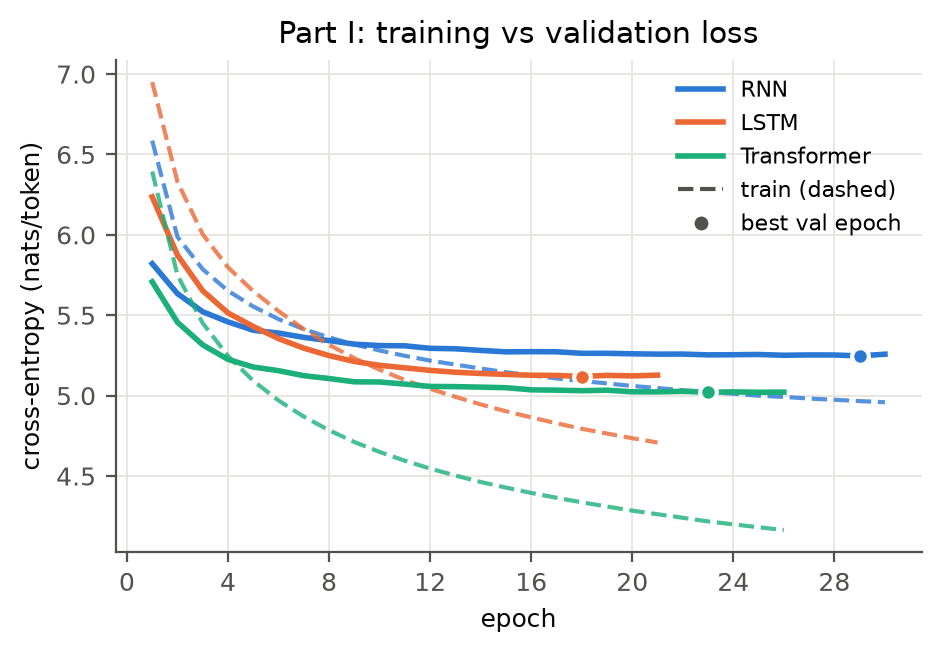
\includegraphics[width=\linewidth]{figures/part1_loss_curves.png}
\end{minipage}\hfill
\begin{minipage}[c]{0.48\linewidth}
  \small\centering
  \resizebox{\linewidth}{!}{%
\begin{tabular}{lrrrr}
  \toprule
  Generated text (5 prompts $\times$ 40 tok) & 3-gram & RNN & LSTM & Transf. \\
  \midrule
  distinct-2 & 0.92 & 0.87 & 0.86 & 0.90 \\
  repeated-trigram fraction & 0.02 & 0.04 & 0.06 & 0.04 \\
  \tok{<unk>} fraction & 0.07 & 0.07 & 0.09 & 0.02 \\
  heading ``='' fraction & 0.04 & 0.14 & 0.14 & 0.05 \\
  \bottomrule
  \end{tabular}}
\end{minipage}
\caption{Left: training (dashed) and validation (solid) CE; the dot marks the best-validation epoch. Right: repetition statistics of continuations under matched decoding (top-$k=40$~\cite{fan2018}, temperature 0.8, 40 new tokens, same seeds; only \tok{<pad>} is banned). Excerpts are in Table~\ref{tab:gen}; full samples are in Appendix~C.}
\label{fig:part1}
\end{figure}

\begin{table}[h]
\centering\footnotesize
\caption{Continuations for the prompts ``in the early years of the war'' / ``he was born in'' (\emph{italics}).}
\label{tab:gen}
\begin{tabularx}{\linewidth}{@{}l>{\raggedright\arraybackslash}X@{}}
\toprule
3-gram & \texttt{. in one season . for the first time . <eos> the family . in the early neolithic builders , he was " . <eos> = = <eos> = = \ldots} / \emph{\texttt{captivity as the film , the first ever " , as the " <unk> in the <unk> @-@ <unk> \ldots}} \\
RNN & \texttt{. <eos> = = = microscopic life = = = <eos> on the other hand , <unk> can be seen in the top of the 20th century . the song was written by her parents \ldots} / \emph{\texttt{march 2006 . <eos> = = = new york = = = <eos> the australian football league games , federer began the second four @-@ yard @-@ winning @-@ touchdown \ldots}} \\
LSTM & \texttt{, the german prerogative was not to be the son of " the <unk> " . the king was also influenced by the <unk> ( croatian @-@ <unk> ) on may 23 , 1863 \ldots} \\
Transformer & \texttt{. <eos> = = = hurricane kenna = = = <eos> in the atlantic ocean , hurricane christine moved to the central pacific ocean . on january 16 , an eye of convection was detected \ldots} / \emph{\texttt{\ldots{} the hurricane produced gusty winds of 140 mph ( 140 km / h ) \ldots}} \\
\bottomrule
\end{tabularx}
\end{table}

\obs{Observations.}
\begin{itemize}
\item \textbf{Prediction quality.} The ranking is Transformer (143.0) $<$ LSTM (156.7) $<$ RNN (176.5) $<$ 3-gram (227.8). Moving from the 3-gram to the RNN gives the largest single drop ($-51$ PPL).
\item \textbf{Convergence.} The Transformer has the lowest validation loss at every epoch. It also overfits most: at its best epoch its validation CE is 0.80 nats above its training CE, versus 0.33 for the LSTM and 0.28 for the RNN, and its training loss keeps falling after validation flattens (Fig.~\ref{fig:part1}). The LSTM starts worst (epoch-1 PPL 511 vs.\ 337 for the RNN) but overtakes the RNN at epoch 6. The RNN converges slowest (best epoch 29) and its validation curve is still noisy at the end.
\item \textbf{Stability.} The RNN alone shows gradient spikes: its pre-clip gradient norm reaches 212.7, against at most 1.7 for the other models.
\item \textbf{Cost.} Wall time per epoch is similar for all three neural models (115--122\,s). Inference throughput (77--91K tok/s) varied by up to 20\% between two identical runs (Transformer: 74K vs.\ 91K tok/s), so we do not rank the neural models by speed. The 3-gram is about $1{,}000\times$ cheaper to ``train'' and about $10\times$ faster to score, but it stores 2.6M entries.
\item \textbf{Generated text} (Table~\ref{tab:gen}).
  \begin{itemize}
  \item The 3-gram produces locally plausible trigrams with no phrase-level coherence (``he was born in captivity as the film'').
  \item The RNN and LSTM produce fluent spans of 5--10 tokens but drift topic within a sentence (the RNN moves from ``australian football league'' to ``federer'' to ``touchdown''). About 14\% of their tokens are section-heading markup.
  \item The Transformer stays on one topic for an entire continuation (hurricane, chart positions, genus/species) and emits the fewest \tok{<unk>} tokens (1.5\%). It still makes local repetitions (``a range of a range of'', ``corpus christi and corpus christi'') and inconsistent facts (``140 mph ( 140 km / h )'', ``debuted at number 1 \ldots{} peaked at number 21'').
  \end{itemize}
  The repetition statistics differ only slightly between models and come from just 200 tokens per model, so we treat them as illustrative.
\end{itemize}

\obs{Possible explanations} (not tested separately).
\begin{itemize}
\item \textbf{Transformer advantage.} Self-attention gives every position direct access to all 64 preceding tokens, which fits the observed topical consistency. However, the Transformer also has the largest backbone (1.10M vs.\ 0.89M for the LSTM and 0.22M for the RNN), so architecture and parameter count are confounded.
\item \textbf{Transformer overfitting.} Its larger train--validation gap suggests higher memorisation capacity on a 2M-token corpus. Every model saw at most about 62M training tokens (30 epochs), well below the roughly 20 tokens per parameter suggested as compute-optimal for 11M-parameter models~\cite{hoffmann2022}, so this is a data-limited regime.
\item \textbf{RNN instability.} The RNN's spikes match the exploding-gradient behaviour of tanh recurrences~\cite{pascanu2013}. Clipping was essential to train it at all, and the instability probably contributes to its slow, noisy convergence.
\item \textbf{Similar epoch times.} About 70\% of each neural model's parameters are in the 28.9K-way softmax layer, which plausibly dominates compute at this scale. The Transformer's parallelism therefore does not show up as faster training at $T=64$ on one GPU.
\end{itemize}
\textbf{Trade-off.} On this budget, the Transformer buys about 9\% lower PPL than the LSTM and clearly better topical consistency at similar wall time. It needs early stopping because it overfits fastest. The n-gram is the only choice when training compute is nearly zero, but it degrades sharply in quality.

%======================================================================
\section{Part II: Embedding variants (LSTM)}
\textbf{Design.} We use the Part~I LSTM and change only the input-embedding table (100-d). Architecture, data, optimiser, seed (the model is re-seeded right before construction), stopping rule and the 30-epoch cap are identical across the three settings:
\begin{itemize}
\item \textbf{Random, trainable.} We reuse the Part~I LSTM.
\item \textbf{Own Skip-gram, frozen}~\cite{mikolov2013}. gensim Skip-gram trained on the WikiText-2 training split only: window 5, 10 negative samples, 10 epochs, min\_count 1, one thread. It covers 100\% of the vocabulary.
\item \textbf{GloVe, frozen}~\cite{pennington2014}. GloVe 6B 100-d (Wikipedia + Gigaword, 6B tokens). It covers 96.2\% of vocabulary types and 94.7\% of training tokens. The 1,103 out-of-vocabulary (OOV) types are dominated by very frequent WikiText markup: \tok{<unk>} (54.6K occurrences), \tok{<eos>} (23.8K), \tok{@-@} (16.9K), \tok{@.@}, \tok{@,@} and \tok{'t}.
\end{itemize}
OOV rows are drawn from $\mathcal{N}(0,\sigma)$, where $\sigma$ is the standard deviation of the pretrained vectors (0.41 for GloVe), and the \tok{<pad>} row is zero. In both frozen settings the \emph{entire} table is fixed, including the random OOV rows, which leaves 8.32M trainable parameters instead of 11.21M.

\begin{table}[h]
\centering\small
\caption{Embedding ablation on the LSTM. The cost of training our own embeddings is reported separately from LM training. Gradient norms are measured before clipping and averaged per epoch.}
\label{tab:part2}
\setlength{\tabcolsep}{4pt}
\resizebox{\linewidth}{!}{%
\begin{tabular}{lrrrrrrrrrr}
\toprule
Input embedding & Test PPL & Val PPL & Val PPL ep1/ep5 & Best/run & Val$-$train CE & Grad norm mean/max & Trainable & LM time to best & Embedding cost & distinct-2 \\
\midrule
Random, trainable & 156.7 & 167.1 & 511 / 228 & 18 / 21 & 0.33 & 0.25 / 1.26 & 11.21M & 2,191\,s & -- & 0.86 \\
\textbf{Own Skip-gram, frozen} & \textbf{141.1} & \textbf{149.7} & 580 / 200 & 18 / 21 & 0.25 & 0.25 / 1.30 & 8.32M & 1,876\,s & 55\,s (1 CPU thread) & 0.89 \\
GloVe 6B, frozen & 153.1 & 162.5 & 653 / 223 & 18 / 21 & 0.20 & 0.25 / 1.62 & 8.32M & 1,897\,s & external (6B tokens) & 0.75 \\
\bottomrule
\end{tabular}}
\end{table}

\begin{figure}[h]
\centering
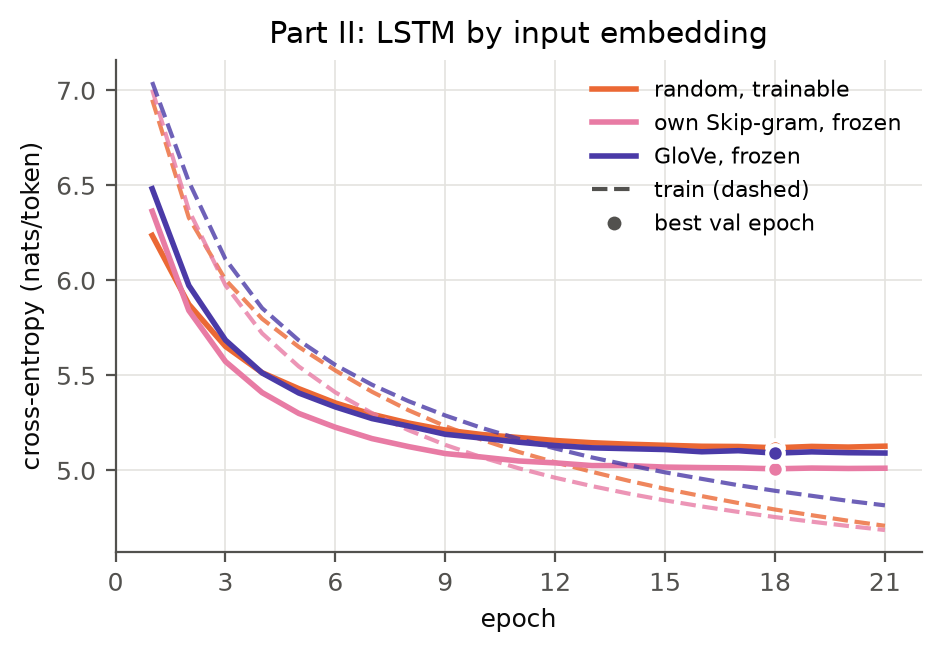
\includegraphics[width=0.49\linewidth]{figures/part2_loss_curves.png}\hfill
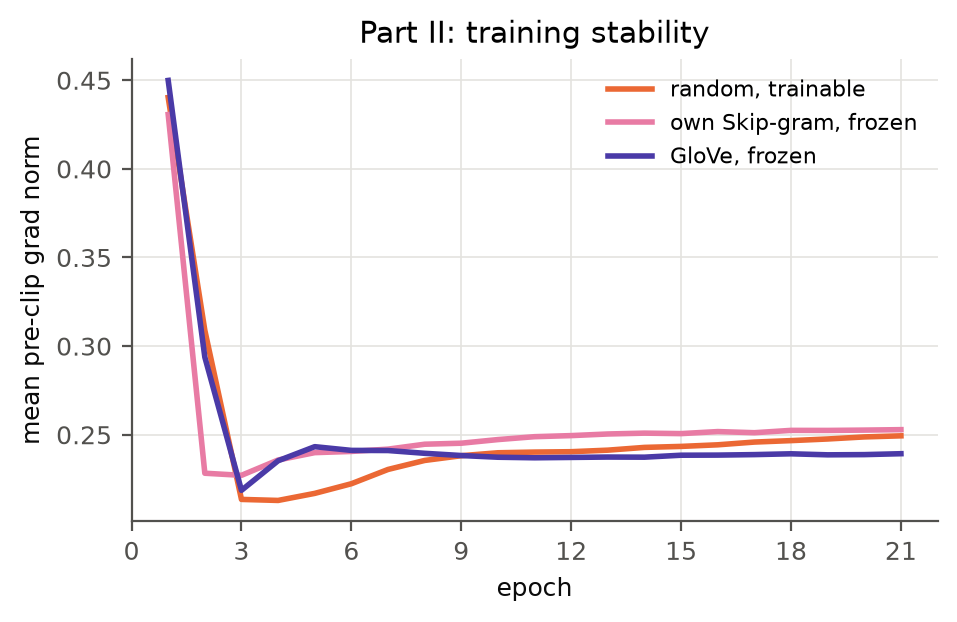
\includegraphics[width=0.49\linewidth]{figures/part2_grad_norm.png}
\caption{Part~II training dynamics. Left: training (dashed) and validation (solid) CE. Right: mean pre-clip gradient norm per epoch.}
\label{fig:part2}
\end{figure}

\obs{Observations.}
\begin{itemize}
\item \textbf{Prediction quality.} Both frozen settings beat the trainable baseline: Skip-gram reduces test PPL by 15.6 ($-10\%$) and GloVe by 3.6. The Skip-gram LSTM (141.1) even edges past the Part~I Transformer (143.0).
\item \textbf{Convergence.} The frozen settings start worse (epoch-1 PPL 580 and 653 vs.\ 511), but Skip-gram overtakes the baseline at epoch 2. All three settings reach their best epoch at 18, and freezing narrows the generalisation gap ($0.33 \to 0.25 / 0.20$ nats).
\item \textbf{Stability.} Gradient behaviour is nearly identical across settings (mean norm 0.25, maximum 1.26--1.62; Fig.~\ref{fig:part2}). Embedding choice does not affect stability here, unlike the architecture choice in Part~I.
\item \textbf{Cost.} Training our own embeddings costs 55\,s, about 3\% of the LM's time to best.
\item \textbf{Generated text.} The GloVe model's samples are the most repetitive (distinct-2 0.75), but 24\% of its sampled tokens are heading markup (``= = = synopsis = = ='' repeated). With only 5 samples, we do not draw conclusions from this.
\end{itemize}

\obs{Interpretation: trainability vs.\ extra data.}
\begin{itemize}
\item \textbf{Why freezing helps.} Freezing removes 2.89M parameters (26\%) that would otherwise be fitted to only 2M tokens. The smaller generalisation gaps are consistent with reduced overfitting, and the Skip-gram result shows that a good fixed initialisation is worth more here than trainability. A plausible mechanism is that Skip-gram gives every word, including rare ones (min\_count $=1$, 10 passes), a vector shaped by its contexts. In the trainable table, rare words receive only a few noisy updates from the LM loss.
\item \textbf{Why GloVe helps less despite its data.} GloVe was trained on about $3{,}000\times$ more text, yet it helps less than Skip-gram on WikiText-2 PPL. Two plausible reasons:
  \begin{enumerate}
  \item The OOV rows are precisely the most frequent structural tokens, so 5.3\% of input tokens enter the LSTM as fixed random vectors that can never be refined.
  \item Skip-gram was trained on exactly the LM's token stream and its tokenization conventions, whereas GloVe reflects a different corpus mixture.
  \end{enumerate}
  The extra data in GloVe therefore does not translate into in-domain prediction, but it does matter for out-of-domain features (Part~III).
\item \textbf{What this design cannot separate.} It cannot fully disentangle ``fixed vs.\ trainable'' from ``initialisation quality''. A pretrained-but-trainable variant would separate the two; we did not run it (Section~\ref{sec:lim}).
\end{itemize}

%======================================================================
\section{Part III: Downstream representation analysis}
\textbf{Task and protocol.} AG News topic classification~\cite{zhang2015} (4 balanced classes) with stratified subsets: 10K train and a disjoint 2K validation set from the official training split, and 2K test from the official test split.
\begin{itemize}
\item \textbf{Tokenization.} Texts are tokenized to mimic WikiText conventions (punctuation and clitics split, \tok{@-@} / \tok{@,@} markers, HTML entities removed), mapped into the LM vocabulary and truncated to 64 tokens. Texts average 44.6 tokens; 6.2\% are truncated and 8.4\% of tokens are \tok{<unk>} (vs.\ 6.2\% on WikiText-2 test).
\item \textbf{Representations.} Every LM stays frozen. A text becomes one fixed-length vector in one of three ways:
  \begin{itemize}
  \item \textbf{last}: the top-layer hidden state at the last non-pad position.
  \item \textbf{mean}: the average of top-layer states over non-pad positions, masked so padding is excluded.
  \item \textbf{emb-mean}: the average of the LSTM's \emph{input} embeddings, used as a context-free reference.
  \end{itemize}
  Right padding never influences these states, because every model is causal.
\item \textbf{Classifier.} All representations share the same classifier family and procedure: standardisation followed by multinomial logistic regression, with $C\in\{0.01, 0.1, 1, 10\}$ selected on validation macro-F1. The test set is scored once. We report 95\% bootstrap confidence intervals (1,000 resamples of the test set) and paired bootstrap tests for the key differences.
\end{itemize}

\begin{table}[h]
\centering\small
\caption{Frozen-LM features with a logistic-regression probe on AG News.}
\label{tab:part3}
\begin{tabular}{lrrlrr}
\toprule
Representation (frozen LM, pooling) & Dim & Test acc. & Test macro-F1 [95\% CI] & F1 Business / Sports & LM test PPL \\
\midrule
LSTM, last & 256 & 0.649 & 0.644 [0.623, 0.663] & 0.48 / 0.79 & 156.7 \\
LSTM, mean & 256 & 0.705 & 0.703 [0.686, 0.723] & 0.60 / 0.83 & 156.7 \\
Transformer, last & 256 & 0.720 & 0.718 [0.700, 0.735] & 0.60 / 0.85 & 143.0 \\
Transformer, mean & 256 & 0.774 & 0.773 [0.755, 0.790] & 0.69 / 0.88 & 143.0 \\
RNN, mean & 256 & 0.730 & 0.727 [0.708, 0.746] & 0.61 / 0.85 & 176.5 \\
LSTM + own Skip-gram (frozen), mean & 256 & 0.791 & 0.790 [0.772, 0.806] & 0.69 / 0.90 & 141.1 \\
\textbf{LSTM + GloVe (frozen), mean} & 256 & \textbf{0.831} & \textbf{0.830 [0.812, 0.847]} & 0.75 / 0.93 & 153.1 \\
LSTM input embeddings, emb-mean (no context) & 100 & 0.674 & 0.672 [0.651, 0.692] & 0.57 / 0.76 & -- \\
\bottomrule
\end{tabular}
\end{table}

\begin{figure}[h]
\centering
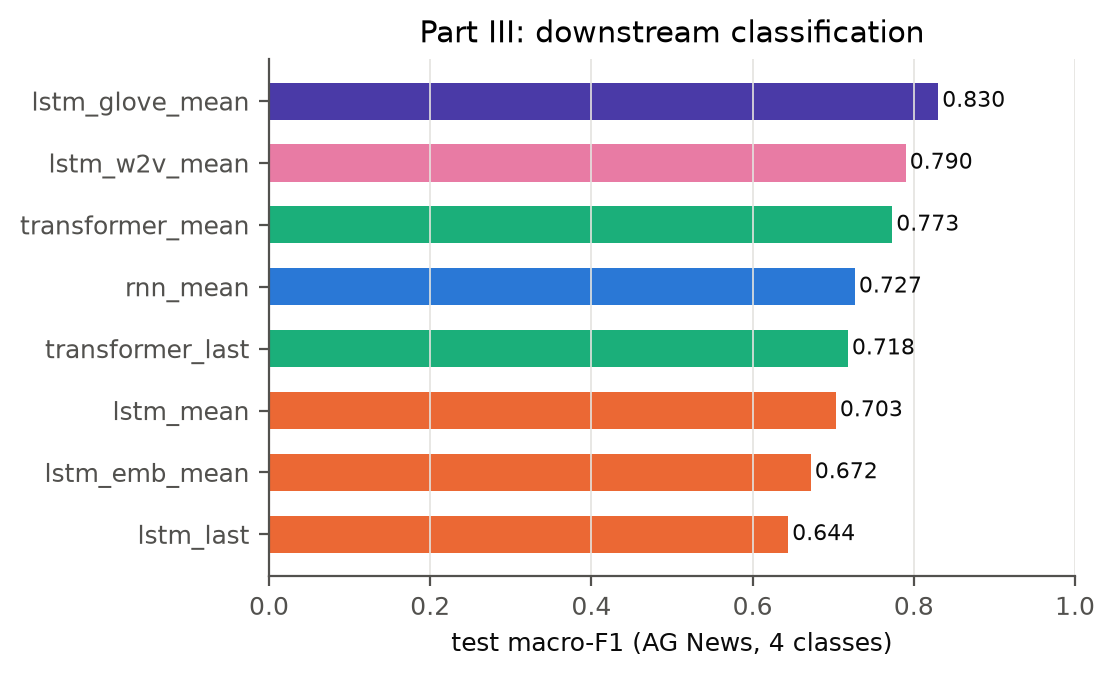
\includegraphics[width=0.49\linewidth]{figures/part3_scores.png}\hfill
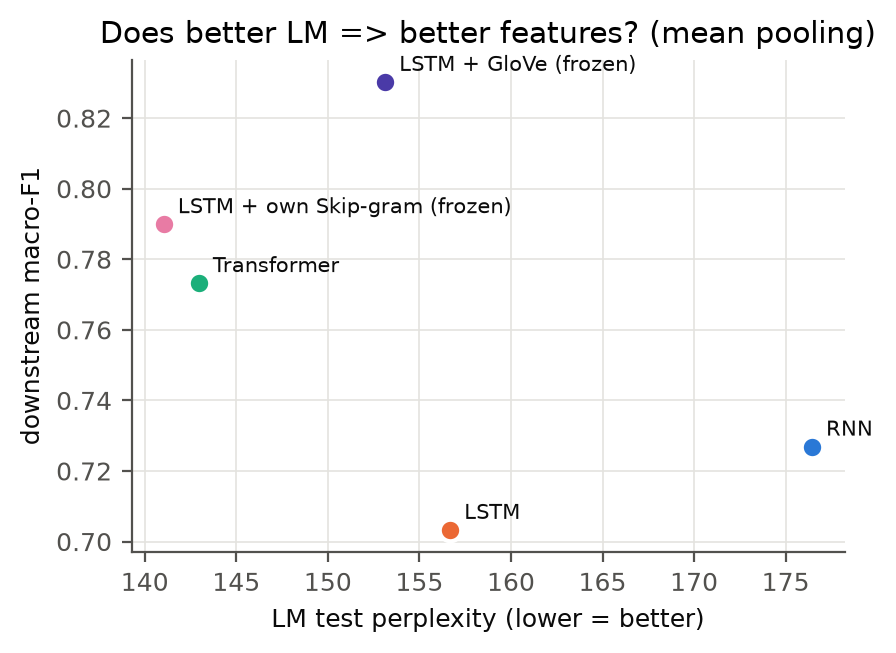
\includegraphics[width=0.49\linewidth]{figures/ppl_vs_downstream.png}
\caption{Left: test macro-F1 of each representation. Right: LM test PPL against downstream macro-F1, one point per LM (mean pooling).}
\label{fig:part3}
\end{figure}

\obs{Observations.}
\begin{itemize}
\item \textbf{Primary comparison: architecture and pooling.}
  \begin{itemize}
  \item The Transformer beats the LSTM under both poolings: $+7.0$ macro-F1 points with mean pooling (paired 95\% CI $[+4.8, +8.9]$) and $+7.4$ with last pooling ($[+5.0, +9.6]$).
  \item Mean pooling beats last-state pooling for both models: $+5.9$ for the LSTM ($[+3.9, +8.0]$) and $+5.5$ for the Transformer ($[+3.7, +7.3]$).
  \item Context helps: LSTM mean states outperform the average of the same model's input embeddings by $+3.1$ ($[+1.0, +5.3]$).
  \end{itemize}
\item \textbf{LM ranking vs.\ downstream ranking.} The two rankings agree only partially. For the five LMs with mean pooling, Spearman $\rho=0.6$ between the PPL rank and the F1 rank ($n=5$, $p=0.28$; Fig.~\ref{fig:part3}, right).
  \begin{itemize}
  \item The Transformer is better than the LSTM on both measures.
  \item The RNN has the \emph{worst} PPL but beats the LSTM downstream ($+2.4$, $[+0.5, +4.2]$).
  \item The largest violation: GloVe ranks only 3rd in PPL but 1st downstream, ahead of Skip-gram ($+4.0$, $[+2.4, +5.6]$), which has the best PPL.
  \item Skip-gram vs.\ Transformer ($+1.7$) is not distinguishable ($[-0.2, +3.5]$).
  \end{itemize}
\item \textbf{Errors.} Business is the hardest class for every representation (F1 0.48--0.75). Its most frequent confusion is with Sci/Tech: 84--117 of the 500 Business test items are predicted as Sci/Tech.
  \begin{itemize}
  \item 121 test items (6\%) are misclassified by all seven contextual representations. Many of these sit on genuine topic boundaries. ``IBM posts broad Q3 revenue growth'' is gold Sci/Tech but predicted Business. ``DaimlerChrysler, GM to team up on hybrid engines'' is gold Business but predicted Sci/Tech.
  \item Some look like label noise: ``Stocks Close Higher on Brokerage Earnings'' and ``Tokyo Stocks Finish 2.6 Percent Higher'' are gold World.
  \item Decisive entity names are often \tok{<unk>} in the WikiText vocabulary (e.g.\ ``Yuganskneftegaz'', ``Hynix''), which removes the strongest cue.
  \item Across representations, GloVe-mean is right where LSTM-last is wrong on 461 items, against 96 in the reverse direction. Typical rescues are sports headlines with misleading surface words, such as ``Red Sox Stumble and Fumble Their Way to Series Lead'' (LSTM-last: Sci/Tech).
  \end{itemize}
\end{itemize}

\obs{Interpretation.}
\begin{itemize}
\item \textbf{Why mean pooling wins.} The last state is trained to predict the \emph{next} token, so it mostly encodes local syntax near the end of the snippet, often just after a full stop. Averaging aggregates the topical words spread across the text.
\item \textbf{Why the rankings disagree.} Lower WikiText-2 PPL is neither necessary nor sufficient for better topic features. Downstream accuracy depends heavily on lexical knowledge of news vocabulary and entities. GloVe acquired this from 6B tokens that include newswire (Gigaword), the same genre as AG News, while PPL measures only in-domain Wikipedia prediction. In-domain Skip-gram helps both measures. The RNN result shows that ranking reversals happen even without external data, which fits a broader point: next-token loss rewards local predictive detail, which is not the same as text-level topic information. We cannot isolate a mechanism for the RNN case from these runs.
\end{itemize}

%======================================================================
\section{Limitations, failure cases, and lessons}\label{sec:lim}
\begin{itemize}
\item \textbf{Single seed and limited timing.} Each configuration was trained once (seed 42), and the MPS kernels are not bit-exact, so small PPL differences (e.g.\ Skip-gram LSTM vs.\ Transformer, 141.1 vs.\ 143.0) are not established. Throughput was timed once per model and varied by up to 20\% between identical runs.
\item \textbf{No per-architecture tuning.} All models share one optimiser setting with a constant learning rate and no schedule. Results describe this matched budget and do not show each architecture's best achievable performance.
\item \textbf{Choices that limit comparability.} Lowercasing, a word-level vocabulary with \tok{<unk>}, and 64-token stateless windows make our PPLs incomparable to the literature. Word-level \tok{<unk>} also hurts transfer to AG News (8.4\% \tok{<unk>}).
\item \textbf{Part II gaps.} We did not run trainable pretrained embeddings, so ``frozen'' and ``good initialisation'' are confounded. GloVe's OOV tokens are concentrated on frequent markup, which disadvantages it for this corpus specifically.
\item \textbf{Part III gaps.} A linear probe on frozen features measures linearly accessible information only, and evaluation uses a 2K-item test subset (95\% CIs of about $\pm1.8$ points). Some ``errors'' are label ambiguity.
\item \textbf{Lessons.}
  \begin{enumerate}
  \item With 2M tokens, regularisation by freezing a good in-domain embedding beat adding trainable capacity.
  \item Gradient clipping was not optional for the vanilla RNN.
  \item Representation quality for a downstream task depends on pooling ($\pm6$ points) and on the lexical coverage of pretraining data at least as much as on next-token PPL.
  \end{enumerate}
\end{itemize}

%======================================================================
{\small
\begin{thebibliography}{99}\setlength{\itemsep}{0pt}
\bibitem{merity2016} S.~Merity, C.~Xiong, J.~Bradbury, R.~Socher. Pointer Sentinel Mixture Models. arXiv:1609.07843, 2016.
\bibitem{kneser1995} R.~Kneser, H.~Ney. Improved backing-off for M-gram language modeling. ICASSP, 1995.
\bibitem{chen1999} S.~F.~Chen, J.~Goodman. An empirical study of smoothing techniques for language modeling. Computer Speech \& Language, 1999.
\bibitem{hochreiter1997} S.~Hochreiter, J.~Schmidhuber. Long short-term memory. Neural Computation, 1997.
\bibitem{vaswani2017} A.~Vaswani et al. Attention is all you need. NeurIPS, 2017.
\bibitem{xiong2020} R.~Xiong et al. On layer normalization in the Transformer architecture. ICML, 2020.
\bibitem{pascanu2013} R.~Pascanu, T.~Mikolov, Y.~Bengio. On the difficulty of training recurrent neural networks. ICML, 2013.
\bibitem{mikolov2013} T.~Mikolov et al. Distributed representations of words and phrases and their compositionality. NeurIPS, 2013.
\bibitem{pennington2014} J.~Pennington, R.~Socher, C.~D.~Manning. GloVe: Global vectors for word representation. EMNLP, 2014.
\bibitem{zhang2015} X.~Zhang, J.~Zhao, Y.~LeCun. Character-level convolutional networks for text classification. NeurIPS, 2015.
\bibitem{hoffmann2022} J.~Hoffmann et al. Training compute-optimal large language models. NeurIPS, 2022.
\bibitem{fan2018} A.~Fan, M.~Lewis, Y.~Dauphin. Hierarchical neural story generation. ACL, 2018.
\bibitem{software} Software: PyTorch; gensim (R.~\v{R}eh\r{u}\v{r}ek, P.~Sojka, 2010); scikit-learn; HuggingFace \texttt{datasets}; matplotlib.
\end{thebibliography}
}

%======================================================================
\clearpage
\appendix
\section*{Appendix A \quad Configuration and reproducibility}
\begin{table}[h]
\centering\small
\begin{tabularx}{\linewidth}{@{}l>{\raggedright\arraybackslash}X@{}}
\toprule
Setting & Value \\
\midrule
Data & WikiText-2 v1 (lowercased); vocab 28,913 from train; windows 64+1, stride 64, no state carry-over \\
Shared LM settings & emb 100, untied output, Adam lr $10^{-3}$, wd 0, batch 32, clip 1.0, $\le$30 epochs, early stop patience 3 (val CE), seed 42 \\
RNN / LSTM & 2 layers, hidden 256, dropout 0.3 (embedding, between layers, output) \\
Transformer & 100$\to$256 projection, learned positions (64), 2 pre-LN blocks, 4 heads, FFN 512, GELU, dropout 0.2, final LayerNorm \\
3-gram & Interpolated Kneser--Ney, $D=0.75$; uniform interpolation at unigram level \\
Skip-gram & gensim 4.4, sg=1, dim 100, window 5, negative 10, 10 epochs, min\_count 1, 1 worker, \texttt{PYTHONHASHSEED=0} \\
Generation & 5 prompts (\texttt{configs/prompts.txt}), top-$k$ 40, $T$ 0.8, 40 tokens, seed $123+i$, context clipped to 64 \\
Part III & AG News 10K/2K/2K stratified (seed 42), max 64 tokens, StandardScaler + LogisticRegression (lbfgs, max\_iter 5000), $C$ by val macro-F1 \\
\bottomrule
\end{tabularx}
\end{table}
{\small Everything is reproduced with \texttt{bash scripts/run\_all.sh} (about 4.5\,h on the hardware above). All hyperparameters are in \texttt{configs/}, and every metrics JSON stores its resolved config and hardware info. See \texttt{README.md} for data access and commands.}

\section*{Appendix B \quad Effect of the training budget (15 vs.\ 30 epochs)}
{\small An earlier run capped at 15 epochs stopped every neural model at epoch 15, so none had converged. We therefore raised the cap to 30 epochs. The ranking is unchanged, and the gains are 1--3\%:}
\begin{table}[h]
\centering\small
\begin{tabular}{lrrrrr}
\toprule
Test PPL & RNN & LSTM & Transformer & LSTM + Skip-gram & LSTM + GloVe \\
\midrule
15-epoch cap & 180.0 & 158.0 & 145.7 & 142.1 & 155.3 \\
30-epoch cap (reported) & 176.5 & 156.7 & 143.0 & 141.1 & 153.1 \\
\bottomrule
\end{tabular}
\end{table}
{\small The Part~III ordering was also stable. With the 15-epoch models the macro-F1 values were GloVe 0.834, Skip-gram 0.789, Transformer-mean 0.760, RNN-mean 0.693, LSTM-mean 0.689 and LSTM-last 0.608. The same Transformer throughput measured 73.9K tok/s in that run, compared with 91.3K here.}

\section*{Appendix C \quad Generated samples (matched decoding)}
\begin{table}[h]
\centering\footnotesize
\begin{tabularx}{\linewidth}{@{}l>{\raggedright\arraybackslash}X@{}}
\toprule
Model & Prompt $\to$ continuation (first 25 tokens) \\
\midrule
3-gram & \texttt{[the history of the city] of sarnia , which was then re @-@ released as an official single " no one wanted to do so , the <unk> and \ldots} \\
RNN & \texttt{[the album was released] by paul mccartney . she was nominated for the uk of the music and <unk> . <eos> = = = = <unk> <unk> = = = \ldots} \\
LSTM & \texttt{[the species is found in] the genus . <eos> = = = chemical bodies = = = <eos> although a protein of cadmium is a dag , the cell is \ldots} \\
Transformer & \texttt{[the album was released] on august 17 , 2006 . " crazy in love " debuted at number 1 on the billboard hot 100 , 2009 . it peaked at number 21 \ldots} \\
Transformer & \texttt{[the species is found in] the united states . the formation of species is a member of the migratory species of species that is particularly in the genus stereum \ldots} \\
LSTM + Skip-gram & \texttt{[the album was released] on cd @-@ rom on july 7 , 2013 , and the video has been released on june 14 , 2003 , which the song was released \ldots} \\
LSTM + GloVe & \texttt{[the album was released] by michael kahne . <eos> = = = synopsis = = = <eos> = = = production = = = <eos> = = = critical reception = = = \ldots} \\
\bottomrule
\end{tabularx}
\end{table}
{\small All samples are in \texttt{results/samples/*.txt}, and the full Part~III error lists are in \texttt{results/samples/part3\_errors.md}.}

\section*{Appendix D \quad Responsible tool and data use}
{\small All datasets are public and are downloaded by the code: WikiText-2 (CC BY-SA), AG News (non-commercial research use) and GloVe (PDDL). None are redistributed in the repository. No API keys or private data are used. \textbf{AI assistance:} the code base (data pipeline, models, training and evaluation scripts) and a first draft of this report were produced with the help of Claude (Anthropic), an AI coding assistant, under my direction. I chose the experimental design, reviewed and ran all experiments, verified the reported numbers against the generated result files, and revised the analysis to reflect my own understanding. \textcolor{red}{[Edit this statement so that it accurately describes your own contribution.]}}

\end{document}
